%% checkpoint1.tex
%% @author farhan haziq

%% ancillaries stuff
\documentclass{vgtc}                        
\ifpdf%                                % if we use pdflatex
  \pdfoutput=1\relax                   % create PDFs from pdfLaTeX
  \pdfcompresslevel=9                  % PDF Compression
  \pdfoptionpdfminorversion=7          % create PDF 1.7
  \ExecuteOptions{pdftex}
  \usepackage{graphicx}                % allow us to embed graphics files
  \DeclareGraphicsExtensions{.pdf,.png,.jpg,.jpeg} % for pdflatex we expect .pdf, .png, or .jpg files
\else%                                 % else we use pure latex
  \ExecuteOptions{dvips}
  \usepackage{graphicx}                % allow us to embed graphics files
  \DeclareGraphicsExtensions{.eps}     % for pure latex we expect eps files
\fi%

%% it is recomended to use ``\autoref{sec:bla}'' instead of ``Fig.~\ref{sec:bla}''
\graphicspath{{figures/}{pictures/}{images/}{./}} % where to search for the images
\usepackage[skip=10pt plus1pt, indent=20pt]{parskip}

\usepackage{microtype}                 % use micro-typography (slightly more compact, better to read)
\PassOptionsToPackage{warn}{textcomp}  % to address font issues with \textrightarrow
\usepackage{textcomp}                  % use better special symbols
\usepackage{mathptmx}                  % use matching math font
\usepackage{times}                     % we use Times as the main font
\renewcommand*\ttdefault{txtt}         % a nicer typewriter font
\usepackage{cite}                      % needed to automatically sort the references
\usepackage{tabu}                      % only used for the table example
\usepackage{booktabs}                  % only used for the table example
\onlineid{0}

%% declare the category of your paper, only shown in review mode
\vgtccategory{Research}

%% author and title
\title{Checkpoint 1: Feeling comfortable with chatbot}
\author{Farhan Haziq}
\affiliation{\scriptsize Department of Computer Science \\ \textit{Colorado State University, Fort Collins, Colorado}}
%% author and title end

%% abstract

\abstract{In this research, we analyses and examine human-chatbot interaction and how the differing design and style of the chatbot affected the users’ acceptance of the bots.%
} 

\CCScatlist{ 
  \CCScat{HCI, Chatbot, Artificial-Intelligence, Emotion, Affective, Connection}%
}
%% abstract end


\begin{document}
\firstsection{Introduction}
\maketitle
Affective computing, as an academic discipline, is in fact, a quite a recent things. In fact, the phrase affective computing wasn’t coined only until the late 1990s \cite{picard_2000}. The recent coalescing of affective computing into a recognized field of study, however, belies the observation that concepts related to both affective computing and artificial intelligence, its parent discipline, can be found many years before either term existed. One of the most en during examples of this is the idea of the Judaism golem; a creature crafted from an ordinary material, such as clay, and brought to life through supernatural which demonstrate human already have those idea even back then.

Emotional bonds are an important, often a productive behavior in human society, it is a process of development of a closeness, interpersonal relationship between two or more entities (whether it be human or otherwise). More often than not, emotional bonds don’t simply arise from an exchange of facial displays, but often emerge through the dynamic give and take of face-to-face interactions. However, in the early 2010s, we are currently seeing the rise of Artificial Intelligences (AI) that allow us human, to interact with them in the like of voice assistant such as Siri and many others. The idea of having some feeling toward a virtual entities aren’t new, it has been part of science fiction trope for ages and with the advancement of AI, it is hard not to overstate the depth, breadth, or pace of change in virtual technology that has gone through for the past half-a-centuries and with the rise of AI. 

Nonetheless. This begs a question, as the AI advanced further, can us human, feel more homely and human-y with these virtual entities like how we do with normal human? This research will attempt to answer the question by letting a participants interact with a chatbot and gather up their conclusions.

%% introduction end

\section{Literature Review and Related Work}

To understand all of this, we also need to look at the book that started
this whole conversation, the eponymously named \emph{Affective
Computing} by Rosalind Picard at Massachusetts Institute of Technology
(MIT) {[}1{]}, published in the year 2000. This book encompass all the
thing that we going to look into.


For this paper, one of the recommended material that I recommend reading
is \emph{Building an AI That Feels} \cite{czerwinski_hernandez_mcduff_2021}, this reading should help in
understanding the context behind the things that we are doing, this
article is written by those cool people at Redmond's \emph{Human
Understanding and Empathy} team for IEEE. The article aren't too long to
read it which mean you could skimmed through it, anyway, the article
provided a lot of insight for me and telling me about the current state
of the AI and related things with it. It also provided some criticism
and countercriticism of AI that have ``emotion.'' The article also
provided the idea and what I should do to ensure that the chatbot I use
are accurate for this purposes.


Next, another reading that should be checked out is \emph{Emotion
Recognition in Human-Computer Interaction}\cite{911197}. The author for this
paper is quite interesting as they are from diverse amount of department
and faculties and not just computer science people, they are also
written by people in linguistics field and philosophical field among
many others. Which then should give this paper a remarkably diverse
perspective from this topic from different sets of lenses. This paper
is, however, a little bit old as it dated back from 2001 and its pretty
long and a bit more technical to read them. As such, this is not the
easiest material to read and understand it. However, this is an
excellent paper that can gives insight on how human emotion can be
interpreted by the machine and the science behind all the emotion behind
human that should be useful in designing the experiment.

Perception is a big part that will play a role in this experiment, this
can be seen in the \emph{Humanizing chatbots: The effects of visual,
identity and conversational cues} \emph{on humanness perceptions}
\cite{GO2019304} where the article that talks about this and how our perception
on their appearances or how they ``behave'' can impact how our
participant might perceive these bots and may alter the result of this
research.

To base the performance of the bot and judge how good they are, this is
where we look to the \emph{Estimating the Impact of `Humanizing'
Customer Service Chatbots} \cite{doi:10.1287/isre.2021.1015} which helps us on how to evaluate and
how to assess the bot's performance and also evaluate the participants
``comfortness'' with the bots. This paper are produced recently, which
should helped with the relevancy of the study.


With all the related work, it should help us to bring this project to a
right directions.


\section{Methodology }
For this purposes. We uses two bots as a way to compare how people will react or feel and perceive  about this. As such, one of the bots is modelled as close as human as possible, this include the usage of jokes, humour, emoji in their reply. 

The second bots will have less of that (i.e.: less human) and their answer will be direct, straightforward and minimal amount of emotions will be used for this bots. The bot’s response time will also be slightly delayed to mimic how long it took for an average human to respond in most messages and make it more realistic.

Finally, there will be no bots at all and instead, a real human will respond to them, the condition given to participants would be divide equally among participant and they will not be told about which kind of bots are they going to talk with (or human) in order to reduce their biasness on this. The participants will then interact with the bot like how they would interact with other people. Right after that, there will be a questionnaire that they will answer on what they feel about those bots, what could be better.

After all that has been done, they will done answer some questionnaire questions and be asked on how they feel on this and gather data from there.


\section{Progress}

Currently, the bots is in training stage and should be ready on checkpoint 2, the questionnaire will also be ready before checkpoint 2. The trainign process can be seen in picture below. The proposal has also been editted to reflec in respond to the commentary last time around.

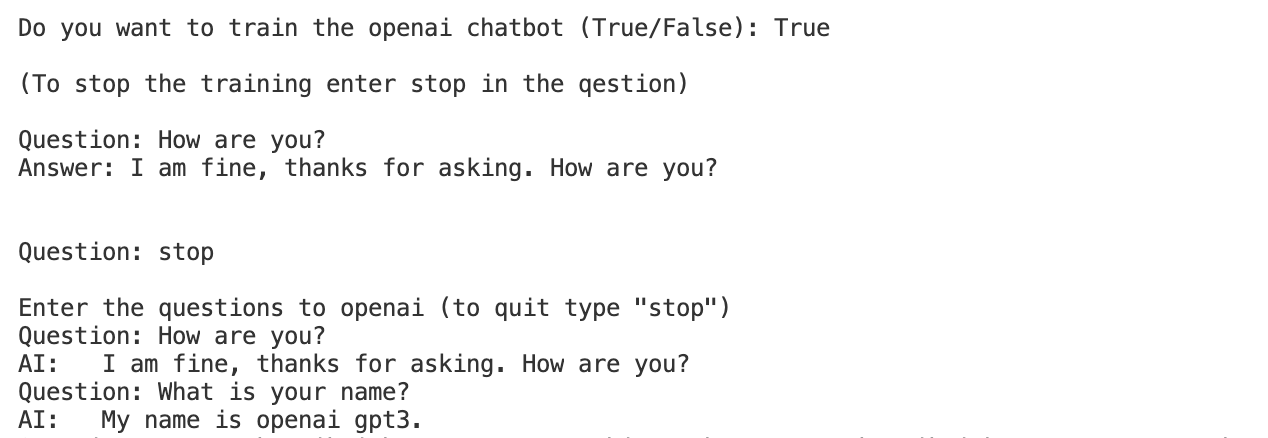
\includegraphics{Openai-gpt3-chatbot-output.png}



%%\acknowledgments{}

%\bibliographystyle{abbrv}
\bibliographystyle{abbrv-doi}
%\bibliographystyle{abbrv-doi-narrow}
%\bibliographystyle{abbrv-doi-hyperref}
%\bibliographystyle{abbrv-doi-hyperref-narrow}

\bibliography{checkpoint1}
\end{document}
